\documentclass[10pt]{article}
\usepackage[margin=0.92in]{geometry}
\usepackage{amsmath,amssymb,booktabs}
\usepackage[T1]{fontenc}
\usepackage{lmodern}
\usepackage{xcolor}
\usepackage{hyperref}
\usepackage{pgfplots}
\pgfplotsset{compat=1.18}
\hypersetup{colorlinks=true,linkcolor=blue,citecolor=blue,urlcolor=blue}
\setlength{\parindent}{0pt}
\setlength{\parskip}{5pt}
\newcommand{\E}{\mathcal{E}}
\newcommand{\M}{\mathcal{M}}
\title{Can Neural Memories Be Merged\\Without Replaying Experience?\\\large A Controlled Pilot and a Representation Constraint}
\author{Richard Shen\\\small Research working draft}
\date{9 October 2026}
\begin{document}
\maketitle
\begin{center}
\small\textbf{Status: synthetic pilot completed; no pretrained LLM evaluated.}\\
Local pre-run protocol freeze; not externally registered or peer reviewed.
\end{center}
\begin{abstract}
We study a restricted memory-composition problem: two parties encode local facts
into fixed-size neural states, and a state-only merger must support queries
requiring evidence from both parties without rereading their histories. We first
state a standard constraint: exact set-union merging is possible precisely when
the encoder's equivalence classes form a congruence for union. We then evaluate
a symmetric residual merger against trained DeepSets and sum, mean, and max
pooling controls in independently sampled six-entity relational worlds. Each
retained state contains 288 float32 coordinates (1,152 payload bytes). Three
fixed-budget fits produce 396,000 predictions across overlapping-evidence
conditions. On the predeclared primary endpoint, known two-hop world-macro
accuracy at overlap probability 0.50, the residual merger scores 78.85\% versus
MAXSET's 79.33\%; the paired difference is -0.47 percentage points with a
conditional 95\% world-bootstrap interval [-1.23, +0.32]. The superiority
hypothesis is unsupported. Joint states substantially outperform private-state
controls, but large fit variability and nonzero idempotence and associativity
defects limit architectural conclusions. The result motivates investigating
representations sufficient for future merges rather than scaling this residual
operator. It establishes neither compression efficiency nor improved LLM memory.
\end{abstract}

\section{A bounded memory-composition question}
An agent may process its own history and then exchange a numerical memory with
another agent. The relevant question is not merely whether the exchange avoids
text. It is whether an output state of unchanged capacity retains distinctions
needed for subsequent queries that neither party can resolve alone.

Let $A$ and $B$ be finite sets of events, $E$ a shared query-blind encoder,
$M$ a merger, and $R$ a reader. We require
\[
s_A=E(A),\quad s_B=E(B),\quad s_{AB}=M(s_A,s_B),\quad
\widehat y=R(s_{AB},q),\quad \operatorname{bytes}(s_{AB})\leq b.
\]
The merger receives only $s_A,s_B$; the reader receives only $s_{AB},q$.
Neither receives raw events, an expanding fragment collection, a reference
answer, or an external lookup table. Shared weights and transient buffers are
accounted separately from the retained per-world state. This restriction is
an evaluation contract, not an efficiency theorem.

Duplicate event tuples represent the same event in this pilot. Independent
repeated observations, paraphrases, trust, timestamp conflicts and deletions
have different semantics and are outside the executed experiment. Its neural
writer is a learned event-set encoder, not a general recurrent language model.

Our executed contributions are an auditable task and comparison, information
controls for joint necessity, and a negative result for one learned merger.
We do not claim the first mergeable neural memory, a new DeepSets construction,
a new algebraic theorem, or a convergent replicated data type.

\section{Related work and the novelty boundary}
Mergeable summaries already formalize compact-summary composition with capacity
and approximation constraints~\cite{summaries}. Deep Sets~\cite{deepsets} and
PointNet~\cite{pointnet} establish permutation-invariant learned representations,
including sum and maximum pooling. Such operators are essential baselines,
rather than properties to rename as a new memory architecture.

Cache Merging~\cite{cache} is a particularly close contemporary precedent. Its
content-addressed KV-fragment collection merges by set union and renders a
deterministic concatenation. It already studies split evidence and latent
reasoning. Adding fragments expands that retained collection; our restricted
question fixes the output-state payload. This distinction is a problem boundary,
not proof of originality or superiority. We refer to its revised v2, not an
earlier near-lossless interpretation of its multi-hop results.

Federated many-to-one Hopfield memory~\cite{hopfield} aggregates Hebbian operators
without centralizing raw samples. Its prototype-recovery objective differs
from the arbitrary relation-binding questions here, but it precludes claiming
operator aggregation itself as new. CRDT convergence additionally requires
compatible order, join and update conditions~\cite{crdt}; a symmetric neural
function with good average answers does not supply those guarantees.

This is a targeted primary-source review, not an exhaustive priority search.
None of these papers was independently reproduced in the present package.

\section{A standard constraint on exact merging}
\textbf{Proposition (union congruence).} An exact merger on the image of $E$
satisfying $M(E(A),E(B))=E(A\cup B)$ for every finite $A,B$ exists if and only if
\begin{equation}
E(A)=E(A')\ \Longrightarrow\ E(A\cup B)=E(A'\cup B)
\quad\text{for every } B.
\label{eq:congruence}
\end{equation}
\emph{Proof.} Necessity follows because an exact merger receives the same two
inputs in both cases. For sufficiency, choose any representative histories of
two states and define the merger by their encoded union. Equation~\ref{eq:congruence}
makes replacing the first representative harmless; commutativity of union gives
the same independence for the second. The operation is therefore well defined.
On reachable states it inherits union's commutativity, associativity,
idempotence and empty-set identity. $\square$

This is a standard quotient-algebra argument, not an original theorem.
It concerns exact state equality, which is stronger than answering a fixed set
of queries equivalently. It does not establish that our learned encoder meets
the condition.

For a counterexample, let distinct events $a,b,c$ have scalar contributions
$1,2,3$ and let $E$ sum distinct events. Then $E(\{a,b\})=E(\{c\})=3$.
Merging with $E(\{a\})=1$ would have to produce both $3$ and $4$.
No state-only postprocessing can always repair this lost distinction.
Conversely, coordinatewise max of max-pooled event features exactly merges
set unions, and the constant-zero encoder also exactly merges. Exact algebra
alone does not imply useful information.

Finite precision adds a separate limit. A $b$-bit state distinguishes at most
$2^b$ histories. Answering arbitrary membership queries over $n$ independent
binary events without error requires at least $2^n$ distinctions, hence
$b\geq n$. This elementary count excludes lossless unlimited-history claims;
it is not a tight neural-memory bound or evidence that this small pilot is
meaningfully compressed.

\section{Frozen experimental design}
\subsection{Worlds, shared evidence, and leakage controls}
Each world contains six entities and two directed functional relations, with
each relation target sampled independently from the six entities. Relations
are not bijections. A fresh entity permutation renames the whole world.
Training and testing share the entity alphabet and query forms, but use
independent seeded world streams. Fresh sampling does not prove exhaustive
absence of repeated finite worlds.

Each evaluation world supplies the same two evidence sets to four distinct
queries: two one-hop and two two-hop queries. A two-hop query asks
$r_2(r_1(s))$, with the other relation used on the second hop. Its critical
edges, if present, are exclusive to opposite parties. Distractors are retained
with probability 0.85 and overlap with probability 0, 0.25 or 0.50. A 0.20
deletion opportunity per query path removes one needed edge from both parties;
shared edges can affect other queries. The realized unknown-label fraction is
23.23--25.50\% across the nine fit-condition cells, not 20\%.

An evaluator-only oracle rejects worlds in which either private party already
determines a known two-hop answer. Each private evidence set must admit at least
two answers under the independently sampled functional-relation model.
This is stricter than merely checking that a direct path lookup is missing.
No ambiguity result, gold intermediate, union event list, ownership label,
world ID or target enters inference. All revisions are zero. Generator
rejection-attempt counts were not retained; this reporting omission is disclosed
in the deviation log and limits auditing of the accepted distribution.

\subsection{Shared learned writer and reader}
An event $(s,r,o,0)$ receives learned entity, relation and revision embeddings.
A key network determines soft routing into 12 slots; a value network produces
24-dimensional nonnegative features. Sum or coordinatewise max pooling of
the routed features, divided by four, forms a $12\times24$ float32 state.
The writer does not receive the eventual query.

The reader normalizes the slots and attends using subject and relation
embeddings. For two-hop queries its predicted first-hop probability vector
produces a weighted entity embedding for the second read. No gold intermediate
is supplied at inference. Two explicit reads and first-hop supervision are
task-specific inductive biases, not discovery of arbitrary reasoning depth.
The shared model has 25,623 parameters.

\subsection{Mergers and fair-comparison scope}
For corresponding slot vectors $a,b\in\mathbb R^{24}$, the candidate is
\begin{align}
u(a,b)&=[a+b,\ |a-b|,\ a\odot b],\\
\alpha(a,b)&=\frac{2m_am_b}{m_a+m_b+10^{-8}},\qquad
m_a=\frac{\|a\|_2}{\sqrt{24}},\\
M_\theta(a,b)&=a+b+\alpha(a,b)f_\theta(u(a,b)).
\end{align}
Here $f_\theta$ is a $72\rightarrow64\rightarrow24$ MLP with a hidden Tanh,
zero-initialized output layer, and 6,232 parameters. The construction is
commutative and preserves the empty input identity. It is not inherently
idempotent or associative.

DeepSets uses $\rho(\phi(a)+\phi(b))$, with two
$24\rightarrow64\rightarrow24$ Tanh MLPs and 6,320 parameters.
SUM and MEAN combine the candidate's sum-pooled states. MAXSET instead
max-pools the same learned event features locally and applies coordinatewise
max to the resulting states. It changes pooling, not shared encoder weights,
input evidence, output shape or precision. It is not max applied to sum states.

Full-union re-encoding references reread deduplicated raw evidence using sum
or max pooling. They are privileged references, not state-only competitors
or guaranteed performance upper bounds. Private A/B, zero, and mismatched-B
states test evidence dependence. Mismatched B comes from the previous world
in each 25-world batch; donor IDs are preserved.

\subsection{Training and one primary decision}
Seeds 11, 23 and 37 each receive 1,500 shared-model steps (batch 64, AdamW
learning rate 0.003, weight decay 0.0001). Four modes cycle equally:
full-union SUM, split SUM, split MEAN and split MAXSET. Training uses one query
per world, two-hop probability 0.70 and overlap probability 0.30, whereas
evaluation uses four shared-context queries.

The shared writer/reader is then frozen. Residual and DeepSets mergers each
receive 1,000 steps on the same seeded stage-two batch stream, learning rate
0.002. The objective is final-answer CE plus 0.30 first-hop CE plus 0.10
relative MSE to the frozen full-union sum state. The MSE denominator is target
mean squared magnitude floored at $10^{-6}$. There is no idempotence penalty.
Union-state teaching and answer labels are privileged training supervision.
Arithmetic baselines lack this additional training; the comparison matches
retained capacity, not total training cost. Final scheduled checkpoints are
used with no test selection or training extension.

For each fit, 1,000 held-out worlds per overlap condition provide 12,000 query
instances. The primary subset is known two-hop queries at overlap 0.50.
We first average eligible correctness within each world, then worlds within
each fit, and then the three learned-minus-MAXSET fit effects equally. Worlds
with no eligible query are excluded using labels and query type alone.

A paired world-cluster percentile bootstrap draws 5,000 resamples (RNG seed
20261008), independently resampling worlds inside each fit. H1 is supported
only if the conditional 95\% interval's lower bound exceeds zero. This interval
conditions on these three fitted models and does not cover a population of
training seeds. Other metrics and contrasts are descriptive.

\section{Results}
\subsection{Primary superiority hypothesis is unsupported}
Table~\ref{tab:fits} shows large variability among fitted models. Residual
accuracy is 78.85\% and MAXSET accuracy 79.33\% after equally averaging fits.
The primary effect is -0.47 percentage points, conditional 95\% interval
[-1.23, +0.32]. The interval crosses zero. We retain the original
superiority hypothesis as unsupported rather than replacing its comparator.
This is not an equivalence test and does not prove identical performance.

\begin{table}[ht]
\centering
\small
\begin{tabular}{rrrrrr}\toprule
Seed & Worlds & Queries & Residual (\%) & MAXSET (\%) & Difference (pp)\\\midrule
11 & 898 & 1475 & 99.05 & 99.39 & -0.33 \\
23 & 881 & 1443 & 86.15 & 89.16 & -3.01 \\
37 & 885 & 1458 & 51.36 & 49.44 & +1.92 \\
\bottomrule\end{tabular}
\caption{Primary known two-hop world-macro outcomes at overlap 0.50. World
and query counts are the eligible counts. All three final fits are retained.}
\label{tab:fits}
\end{table}

\begin{table}[ht]
\centering\small
\begin{tabular}{lrrrrr}\toprule
Method & K2 macro (\%) & All (\%) & Known (\%) & Unknown recall (\%) & ECE\\\midrule
Symmetric residual & 78.85 & 78.10 & 84.12 & 60.33 & 0.029 \\
DeepSets & 58.31 & 64.53 & 68.14 & 53.72 & 0.052 \\
SUM & 74.18 & 76.20 & 81.33 & 61.04 & 0.027 \\
MAXSET & 79.33 & 78.64 & 85.00 & 59.87 & 0.031 \\
MEAN & 73.69 & 76.24 & 81.04 & 62.06 & 0.028 \\
A only & 5.85 & 44.42 & 34.58 & 74.16 & 0.362 \\
B only & 5.77 & 45.43 & 35.71 & 74.82 & 0.355 \\
Zero state & 0.00 & 25.03 & 0.00 & 100.00 & 0.704 \\
Swapped B & 16.15 & 30.93 & 31.59 & 29.20 & 0.412 \\
Union SUM (replay) & 77.74 & 78.26 & 83.85 & 61.73 & 0.026 \\
Union MAX (replay) & 79.33 & 78.64 & 85.00 & 59.87 & 0.031 \\
\bottomrule\end{tabular}
\caption{Descriptive equal-fit averages at overlap 0.50. K2 macro is known
two-hop world-macro accuracy. Other accuracy entries average query-level fit
metrics. ECE uses ten fixed-width bins. Replay references have raw-event access.}
\label{tab:methods}
\end{table}

MAXSET is the strongest evaluated non-replay merger on the primary mean.
The residual exceeds SUM and MEAN descriptively, but these receive less total
training and were not the primary contrast. DeepSets scores 58.31\%; its poor
result under this fixed budget does not establish an optimal DeepSets comparison.
The residual's addition initialization and identity are favorable inductive
biases, but their causal contributions were not separately ablated.

\subsection{Joint evidence matters; fit quality remains a bottleneck}
Private A and B score 5.85\% and 5.77\% on primary queries, zero state 0\%,
and mismatched B 16.15\%. These controls and the private-ambiguity checks
support dependence on correctly paired distributed evidence in this task.
They do not establish out-of-distribution language reasoning or absence of
every possible shortcut. Zero-state overall accuracy instead reaches 25.03\%
by predicting unknown, illustrating why the known-answer primary subset matters.

Full-union MAX re-encoding matches MAXSET's predictions, as expected from its
pooling algebra. Full-union SUM scores 77.74\%, below the residual mean;
reader imperfections make re-encoding a reference rather than an upper bound.
The substantial seed-37 failure also occurs in privileged references, so
attributing all lost accuracy to the merger would be unjustified.

\begin{figure}[ht]
\centering
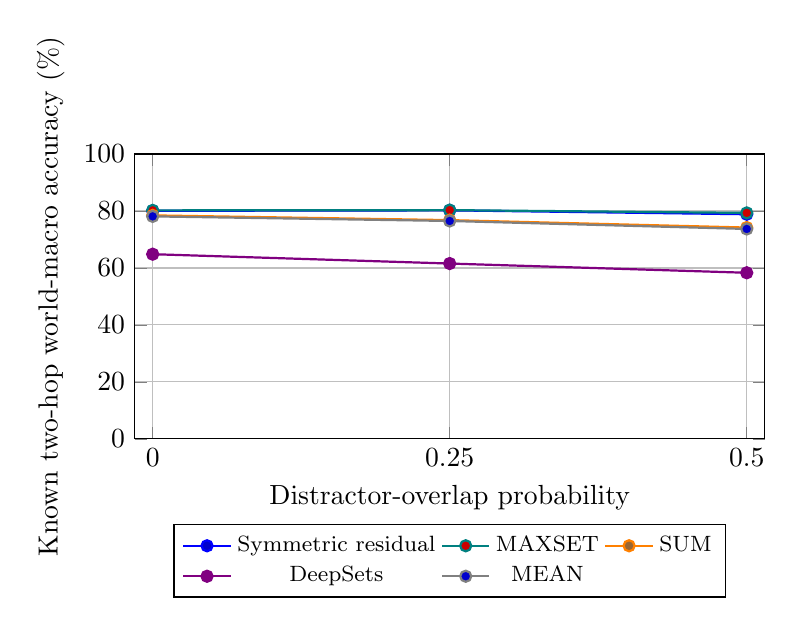
\begin{tikzpicture}
\begin{axis}[width=0.79\linewidth,height=5.2cm,xmin=-0.015,xmax=0.515,
ymin=0,ymax=100,xtick={0,0.25,0.5},xlabel={Distractor-overlap probability},
ylabel={Known two-hop world-macro accuracy (\%)},legend style={font=\footnotesize,
at={(0.5,-0.30)},anchor=north,legend columns=3},grid=major]
\addplot+[color=blue,mark=*,thick] coordinates {(0.0,80.0592) (0.25,80.2303) (0.5,78.8538)};
\addlegendentry{Symmetric residual}
\addplot+[color=teal,mark=*,thick] coordinates {(0.0,80.2092) (0.25,80.2996) (0.5,79.3275)};
\addlegendentry{MAXSET}
\addplot+[color=orange,mark=*,thick] coordinates {(0.0,78.4530) (0.25,76.7912) (0.5,74.1814)};
\addlegendentry{SUM}
\addplot+[color=violet,mark=*,thick] coordinates {(0.0,64.8330) (0.25,61.5492) (0.5,58.3149)};
\addlegendentry{DeepSets}
\addplot+[color=gray,mark=*,thick] coordinates {(0.0,78.1036) (0.25,76.4959) (0.5,73.6915)};
\addlegendentry{MEAN}
\end{axis}\end{tikzpicture}
\caption{Descriptive equal-fit means across overlap. The primary comparison
uses only overlap 0.50. These points have substantial fit variability
(Table~\ref{tab:fits}) and no plotted uncertainty interval.}
\label{fig:overlap}
\end{figure}

\subsection{Symmetry does not give a convergent memory}
The candidate and DeepSets have zero observed commutativity defect, but
substantial idempotence and associativity defects (Table~\ref{tab:algebra}).
The normalized defect is the square root of output MSE divided by input-A
mean squared magnitude floored at $10^{-6}$, averaged over evaluation batches
and then fits. State agreement is separate from answer correctness.

\begin{table}[ht]
\centering\small
\begin{tabular}{lrrr}\toprule
Method & Commutativity & Idempotence & Associativity probe\\\midrule
Symmetric residual & 0 & 0.636 & 0.1486 \\
DeepSets & 0 & 0.8532 & 0.1548 \\
SUM & 0 & 1 & 4.627e-08 \\
MAXSET & 0 & 0 & 0 \\
MEAN & 0 & 0 & 0.1338 \\
\bottomrule\end{tabular}
\caption{Relative state RMSE at overlap 0.50. The associativity probe is weak:
its third state is a one-row roll, so 75\% coincide with A. This is not
same-world three-party semantic integration.}
\label{tab:algebra}
\end{table}

SUM's small associativity defect is floating-point rounding; MAXSET's three
defects are zero in the executed probe. MEAN is idempotent but not associative.
No same-world three-party answer test or within-party duplication test was run.
The observed properties do not confer a neural CRDT guarantee.

\section{Interpretation, limitations, and next research gate}
The pilot demonstrates learned, state-only joint answering within its tiny
task, but does not establish that a new merger improves the strongest simple
baseline. H1 is unsupported, and the additional learned operator should not
be scaled on a claimed superiority result. A narrow negative result cannot
refute all possible mergeable neural-memory architectures either.

The retained payload is 1,152 bytes, while two inputs require 2,304 bytes before
output and temporary allocations. Each fit's checkpoint contains all three
networks and occupies 168,469 serialized bytes. CPU execution uses one thread;
the locked training/evaluation run takes 137.7 seconds. Component timings
exclude encoding and are descriptive, not end-to-end efficiency evidence.
A direct table can store this six-entity world in far fewer than 1,152 bytes;
the pilot therefore does not test a persuasive compression bottleneck.

All conclusions are limited to shared weights, a shared small vocabulary,
two fixed relation types, two-hop query forms and exact tuple identity.
Corrections, forgetting, temporal conflicts, trust, independently learned
encoders, natural-language semantics and pretrained LLM integration remain
unexecuted. Three fits also show considerable fit-to-fit performance variability;
training and test-stream contributions to this variability were not isolated.
The conditional bootstrap does not erase it. Sampling rejection counts are
missing, and future studies should retain them.

A stronger next question is whether a representation preserves distinctions
needed by \emph{future unions}, beyond its current local queries. It follows
from Equation~\ref{eq:congruence} that local sufficiency alone need not ensure
merge sufficiency. A new protocol should compare separately optimized strong
pooling writers, an explicit relation-table reference, meaningful fixed-byte
capacity sweeps, and adversarial locally indistinguishable histories. Only
after a stable benefit should it add semantic multi-party merges, subsequent
writes, and an actual language backbone. This is a proposed direction, not a
post-hoc successful result or a newly proved learning principle.

\section*{Reproducibility and research assistance}
The local input freeze was created on 2026-10-08 at
16:32:32.407124 UTC (9 October in Asia/Shanghai), before fitting.
The archive contains frozen configuration/source/dependencies/tests,
per-query probabilities and donor IDs, all final checkpoints, training traces,
output hashes, an independent statistical reconstruction, and a deviation log.
The audit recomputes metrics from saved predictions and checks recorded private
ambiguity counts; raw fact sets and per-world latent states were not archived
for independent row-level recomputation. Frozen code and seeds permit future
regeneration, which was not performed by this audit.
Nineteen pre-run checks cover information boundaries, private ambiguity,
gradient paths, grouping and algebraic examples. A local checksum freeze is
not external registration. Machine-readable evidence takes precedence over
rounded tables. There was no test-driven hyperparameter search, checkpoint
selection or training extension in the executed run.

AI assistance was used for literature review, implementation, adversarial
checks and drafting. Author review and independent replication remain needed
before submission. The package is a research working draft, not a completed
LLM study or a claim of publication readiness.

\begin{thebibliography}{9}
\bibitem{cache} C. Baquero and L. Brito.
\emph{Cache Merging as a Convergent Replicated State for Multi-Agent Latent Reasoning}.
arXiv:2607.01308, v2, 2 October 2026.
\href{https://arxiv.org/abs/2607.01308v2}{Primary source}.
\bibitem{hopfield} A. Alessandrelli et al.
\emph{A Federated Many-to-One Hopfield Model for Associative Neural Networks}.
arXiv:2603.19902, 2026.
\href{https://arxiv.org/abs/2603.19902}{Primary source}.
\bibitem{deepsets} M. Zaheer et al. \emph{Deep Sets}. NeurIPS, 2017.
\href{https://arxiv.org/abs/1703.06114}{Primary source}.
\bibitem{pointnet} C. R. Qi et al.
\emph{PointNet: Deep Learning on Point Sets for 3D Classification and Segmentation}.
CVPR, 2017. \href{https://arxiv.org/abs/1612.00593}{Primary source}.
\bibitem{crdt} M. Shapiro et al.
\emph{A Comprehensive Study of Convergent and Commutative Replicated Data Types}.
INRIA Research Report RR-7506, 2011.
\href{https://dsf.berkeley.edu/cs286/papers/crdt-tr2011.pdf}{Original report mirror}.
\bibitem{summaries} P. K. Agarwal et al. \emph{Mergeable Summaries}.
PODS 2012; ACM TODS, 2013.
\href{https://doi.org/10.1145/2500128}{Publication};
\href{https://users.cs.duke.edu/~pankaj/publications/papers/merge-summ.pdf}{Author copy}.
\end{thebibliography}
\end{document}
